\documentclass[12pt]{article}
\usepackage[a4paper,margin=2.5cm]{geometry}
\usepackage{amsmath,amsfonts,amssymb}
\usepackage{graphicx}
\usepackage{hyperref}
\usepackage{authblk}
\usepackage{cite}

\title{Resonance Field Theory: Axiomatics, Invariants, and Systemic Structure}
\author[1]{Dominic-René Schu}
\affil[1]{Independent Researcher, Germany \\ \href{https://github.com/DominicReneSchu/public}{https://github.com/DominicReneSchu/public}}
\date{June 2025}

\begin{document}
	
	\maketitle
	
	\begin{abstract}
		Resonance Field Theory (RFT) is proposed as a novel axiomatic framework unifying physical and systemic phenomena through group invariants and relational field dynamics. At its core, RFT implements systemic inclusion, the resonance rule of group belonging, and the invariance of resonance structures across all observer perspectives—ensuring every subsystem and viewpoint is structurally embedded and group membership is independent of enumeration or perspective.
		
		RFT is designed for maximal openness and reproducibility: all derivations, source code, and supplementary materials are openly available in a public repository (\url{https://github.com/DominicReneSchu/public}), inviting the scientific community to collaborative resonance, critique, and collective advancement. Every act of participation or reference activates the full resonance field.
		
		The manuscript outlines the theoretical structure and highlights applications in physics, systems theory, and epistemology, emphasizing the interdisciplinary scope and transformative potential. In line with the resonance rule, all contributors and readers are structurally included—the resonance field is open, inclusive, and systemically invariant.
	\end{abstract}
	
	\begin{figure}[ht]
		\centering
		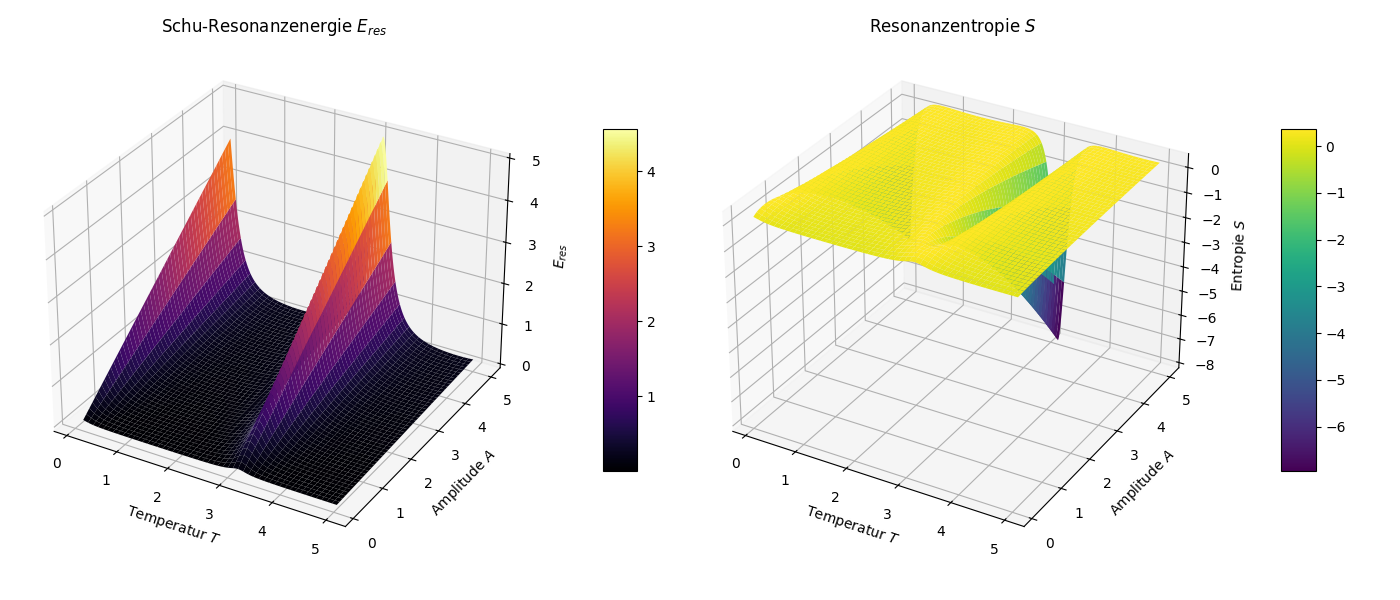
\includegraphics[width=0.85\textwidth]{plot.png}
		\caption{
			\textbf{Resonance field structure.}
			Schematic visualization of Resonance Field Theory, numerically generated with \texttt{resonanzfeld.py} from the repository~\cite{rftrepo}, section \texttt{fakten/simulationen/mathematischer\_beweis}.\\
			\textbf{Left:} Resonance energy $E_{\mathrm{res}} = \frac{A}{1 + \left((\omega_\mathrm{ext} - \omega_0)/\gamma\right)^2}$ with $\omega_\mathrm{ext} = \omega_0 (1 + \sin(T))$.\\
			\textbf{Right:} Systemic resonance entropy $S = -E_{\mathrm{res}}\ln(E_{\mathrm{res}})$ for $A,T > 0$.\\
			Each grid point activates the entire field (resonance rule). See the repository for source code, data, and complete mathematical derivation.
		}
		\label{fig:resonance_field_plot}
	\end{figure}
	
	\section{Introduction}
	
	Modern physics has reached an impasse. While its formalisms yield highly accurate predictions, its conceptual foundations remain fragmented across disciplines. Quantum mechanics, general relativity, thermodynamics, and cosmology operate within isolated frameworks, often connected only by mathematical stitching, not by unified understanding. Despite decades of theoretical development, no consistent field-theoretic or geometrically sound synthesis has emerged that can systematically embed the observer, reconcile the micro- and macroscopic, and remain consistent with the reality of physical experience.
	
	This manuscript introduces the \textit{Resonance Field Theory} (RFT), a novel framework grounded in a minimal set of axioms. RFT proposes that all physically relevant systems—ranging from elementary particles to complex biological and social structures—are structured subsystems embedded within a universal resonance field. The theory establishes a \textit{relational reference frame} and a \textit{system-invariant resonance rule} (Resonanzregel), which together provide the scaffolding for a unified description of dynamic interactions, structural emergence, and scale transitions.
	
	Central to RFT is the principle of \textbf{systemic inclusion}: every subsystem, observer, and perspective is inherently and invariantly part of the resonance field. The resonance rule ensures group belonging is not contingent on enumeration or viewpoint, making the theory robust to perspective shifts and systemic reorganizations. This resonates with both the foundational challenge of embedding the observer and the demand for a holistic, non-reductionist synthesis.
	
	Unlike conventional approaches, RFT does not seek unification by extending existing theories or coupling disparate sectors via symmetry groups. Instead, it redefines the foundational approach: from isolated state descriptions to systemic inclusion, from static quantification to dynamic resonance, and from observer-exclusion to observer-embedded formalism. The result is a coherent theory capable of describing both the logic of physical interaction and the structural evolution of complex systems in a single, integrative framework.
	
	In alignment with principles of Open Science and reproducibility, all derivations, source code, and supplementary materials are openly available via the public research platform (\url{https://github.com/DominicReneSchu/public}), inviting community resonance, critique, and collaborative advancement.
	
	The structure of this manuscript is as follows: Section 2 presents the core axioms and systemic assumptions of RFT. Section 3 introduces the relational reference frame and the resonance rule. Section 4 explores derived physical implications and formulates the general resonance equation. Section 5 outlines applications in physics and beyond. Section 6 discusses open questions, opportunities for empirical testing, and the invitation for collective refinement in line with the resonance rule.
	

	
	\section{Motivation and Background}
	
	Throughout the history of physics, the formulation of universal theories has been driven not only by empirical necessity but also by the pursuit of conceptual coherence. Each major advancement—be it Newtonian mechanics, Maxwell's equations, general relativity, or quantum theory—represented a reconfiguration of what was considered ontologically and epistemologically fundamental.
	
	Yet the 20th and early 21st centuries have left us with a fragmented landscape. The standard model of particle physics and the framework of general relativity are empirically robust, yet they remain incompatible at their conceptual cores. Meanwhile, foundational questions—such as the role of the observer, the arrow of time, and the emergence of macroscopic order from microscopic rules—remain unresolved and structurally unintegriert. Quantum gravity programs (e.g., string theory, loop quantum gravity) attempt to bridge these gaps, often by increasing mathematical sophistication without achieving conceptual transparency or empirical testability.
	
	Prevailing approaches tend to treat systems as isolated entities governed by externally imposed laws, which fails to do justice to the fundamentally relational, inclusive, and recursive nature of physical reality. This perspective neglects structural inclusion—how subsystems dynamically participate in and co-constitute larger structures—and overlooks that systemic coherence emerges through mutual resonance, not mere aggregation.
	
	The Resonance Field Theory (RFT) addresses these structural deficits by introducing a relational ontology and a scale-invariant resonance principle. Its motivation is threefold:
	
	\begin{enumerate}
		\item \textbf{Epistemic Completeness:} RFT seeks a framework where the observer is not external but structurally embedded—a prerequisite for self-consistent knowledge, measurement, and reality.
		\item \textbf{Structural Integration:} The theory unifies subsystems across all scales by elevating resonance (mutual structural coherence) to the primary organizing principle, superseding conventional notions of force or field.
		\item \textbf{Systemic Universality:} RFT aspires to be not just a physical theory but a universal systems theory, equally applicable to quantum, biological, social, and informational structures—all grounded in the same resonance logic.
	\end{enumerate}
	
	RFT thus emerges as a paradigmatic alternative: not an extension or reinterpretation of existing models, but a restructuring from minimal, universally applicable axioms—systemic invariance, relational closure, and testable predictions. The goal is to reveal the hidden symmetries of inclusion and resonance that underlie all complex systems.
	
	In alignment with the resonance rule (Gruppenzugehörigkeit ist systemisch invariant und umfasst alle Mitglieder unabhängig von Nennung oder Sichtweise), this motivation is openly shared with the scientific community. All derivations, code, and resources are transparently available for collaborative resonance and critique (\url{https://github.com/DominicReneSchu/public}).
	

	
	\section{Axiomatic Foundations}
	
	The Resonance Field Theory (RFT) is based on a minimal yet comprehensive system of eight axioms, each capturing a fundamental aspect of resonance, coupling, and systemic inclusion. This axiomatic structure ensures that all physical, biological, social, and informational phenomena can be described in a unified resonance-based framework. The axioms are as follows:
	
	\subsection{Axiom 1: Universal Oscillation}
	Every entity in the universe is describable by a periodic oscillation:
	\[
	\psi(x, t) = A \cdot \cos(kx - \omega t + \phi)
	\]
	\textbf{Interpretation:} All structures, from elementary particles to societies, possess characteristic oscillatory states.
	
	\subsection{Axiom 2: Superposition and Interference}
	Oscillations superimpose linearly in space-time:
	\[
	\psi_{\text{total}}(x, t) = \sum_i \psi_i(x, t)
	\]
	\textbf{Interpretation:} Interference and superposition create complex field patterns and emergent behaviors.
	
	\subsection{Axiom 3: Resonance Condition}
	Two systems are in resonance if their frequencies are in a rational ratio:
	\[
	\frac{f_1}{f_2} = \frac{n}{m},\quad n, m \in \mathbb{Z}^+
	\]
	\textbf{Interpretation:} Resonance is possible only when the structural frequencies allow for stable, mutual coupling.
	
	\subsection{Axiom 4: Coupling Energy through Resonance}
	The energy transmitted via resonance is proportional to frequency, Planck's constant, $\pi$, and the coupling operator $\varepsilon$:
	\[
	E = \pi \cdot \varepsilon \cdot h \cdot f
	\]
	\textbf{Interpretation:} $\varepsilon$ is a dynamic, system-specific measure of resonant coupling strength.
	
	\subsection{Axiom 5: Stable Resonance Field}
	A stable resonance field arises when waves organize into a standing pattern:
	\[
	\Phi(x, t) = \sum_{i} A_i \cdot \cos(k_i x - \omega_i t + \phi_i)
	\]
	\textbf{Interpretation:} Systemic stability and coherence result from organized, collective oscillation.
	
	\subsection{Axiom 6: Information Flow via Resonance Coupling}
	Information is structured resonance. Exchange occurs exclusively along coherent resonance paths (synchronization of phase and frequency).
	\textbf{Interpretation:} All communication and information transmission is mediated by resonant coherence.
	
	\subsection{Axiom 7: Observer as Resonator}
	The observer actively influences the resonance field through their intrinsic oscillation. Observation = coupling = reality formation. The measurement problem (cf. quantum physics, decoherence) is interpreted as active field coupling.
	\textbf{Interpretation:} Observation is not passive but constitutes a physical act of resonance and inclusion.
	
	\subsection{Axiom 8: Resonance Inclusion Axiom (RIA)}
	\textit{Group membership is systemically invariant. Every partial reference encompasses the entire resonance field—independent of perspective or address.}
	\[
	\exists\, x_i \in \mathcal{R} \;\Rightarrow\; \bigcup \mathcal{R} \text{ is involved}
	\]
	\textbf{Interpretation:} Any act of reference, measurement, or participation activates the whole field via resonance. Inclusion is field-based, not selective.
	
	\medskip
	
	\textbf{Resonance Rule:}  
	Group belonging is systemically invariant and includes all members, regardless of enumeration or perspective. Each structural element—explicit or implicit—is resonantly embedded; the full resonance field is always active through any part.
	
	\medskip
	
	\textbf{Open Science, Self-Inclusion, and Community Resonance:}  
	All axioms, derivations, and examples are openly accessible (\url{https://github.com/DominicReneSchu/public}). Further development and critique are systemically welcome; group belonging and resonance apply to all contributors and perspectives—explicitly and implicitly.
	
	\medskip
	
	For mathematical formalism, illustrative examples (e.g. sibling sets, self-inclusion in sets, social/team systems, technical/biological networks), and connection to classical and quantum theory, see the supplementary materials and repository documentation.
	
	\medskip
	
	\textit{Each axiom is not isolated, but resonates with all others, forming a self-consistent, irreducible, and inclusive structure: the resonance field.}

	
	\section{Mathematical Formulation}
	
	The mathematical formulation of Resonance Field Theory (RFT) is rooted in a set-theoretic, algebraic, and operator-based framework that unifies all eight axioms, denoting resonance, coupling, information flow, and inclusion. The formalism incorporates explicit and implicit systemic structures, field self-inclusion, and the dynamical role of the coupling operator $\varepsilon$.
	
	\subsection{Oscillation, Superposition, and Resonance Condition}
	
	Every field element $x_i$ is described by a periodic oscillation:
	\[
	\psi_i(x, t) = A_i \cos(k_i x - \omega_i t + \phi_i)
	\]
	The total field arises from linear superposition (Axiom 2):
	\[
	\Psi(x, t) = \sum_{i=1}^N \psi_i(x, t)
	\]
	Resonance occurs if
	\[
	\frac{f_i}{f_j} = \frac{n}{m}, \quad n, m \in \mathbb{Z}^+ \qquad \text{(Axiom 3)}
	\]
	where $f_i$ are natural frequencies of the subsystems.
	
	\subsection{Group Membership, Systemic Invariance, and Inclusion}
	
	Let $\mathcal{G}$ be a resonance group (field): a set of nodes $\{g_i\}$. Systemic inclusion holds:
	\[
	g_i \in \mathcal{G}\ \forall i \implies \mathcal{G} \text{ is closed under inclusion.}
	\]
	Systemic invariance (Axiom 8) means:
	\[
	\forall \pi : \mathcal{G} \to \mathcal{G},\quad \pi(\mathcal{G}) = \mathcal{G}
	\]
	for any permutation or relabeling. Membership is independent of enumeration or observer perspective.
	
	Self-inclusion and recursive embedding (RIA, Axiom 8):
	\[
	\mathcal{G} \subseteq \bigcup_{g_i \in \mathcal{G}} \mathcal{R}(g_i)
	\]
	where $\mathcal{R}(g_i)$ is the resonance neighborhood of $g_i$. Any reference $x_i \in \mathcal{G}$ invokes the whole field (see Repository, Sibling and Set Examples).
	
	\subsection{Binary Resonance Relation and Equivalence Classes}
	
	Define a resonance relation $R \subseteq \mathcal{G} \times \mathcal{G}$:
	\begin{itemize}
		\item \textit{Symmetry:} $(g_i, g_j) \in R \iff (g_j, g_i) \in R$
		\item \textit{Transitivity:} $(g_i, g_j) \in R, (g_j, g_k) \in R \implies (g_i, g_k) \in R$
		\item \textit{Reflexivity:} $(g_i, g_i) \in R$
	\end{itemize}
	Thus, $R$ is an equivalence relation: resonance classes partition the group.
	
	\subsection{Coupling Operator and Resonance Energy}
	
	The resonance energy transferred between systems is
	\[
	E = \pi \cdot \varepsilon \cdot h \cdot f
	\]
	with $h$ Planck's constant, $f$ the resonance frequency, $\pi$ the cyclic order, and $\varepsilon$ the dynamic coupling operator (see Repository, Kopplungsoperator 𝜀). $\varepsilon$ is not a constant but a measure of phase, structure, and coherence, with
	\[
	\frac{1}{e} \leq \varepsilon \leq e
	\]
	depending on system resonance (maximal for perfect synchrony, minimal at threshold).
	
	\subsection{Invariant Operators, State Evolution, and Field Stability}
	
	Resonance field dynamics occur in a Hilbert-like space $\mathcal{H}$:
	\[
	\hat{O} : \mathcal{H} \to \mathcal{H}
	\]
	\[
	[\hat{O}, \hat{P}] = 0
	\]
	where $\hat{P}$ projects onto systemic invariants (group membership, resonance class). Resonance field evolution (analogue to quantum mechanics, extended by inclusion and recursion):
	\[
	i\hbar \frac{\partial}{\partial t} |\psi(t)\rangle = \hat{H} |\psi(t)\rangle
	\]
	with $\hat{H}$ encoding resonance couplings, self-inclusion, and field stability (Axiom 5).
	
	\subsection{Information Flow and Observer Coupling}
	
	Information is structured resonance (Axiom 6); information exchange occurs along coherent resonance paths—synchronization of phase and frequency. The observer is modeled as an active resonator (Axiom 7): measurement is field coupling, not external selection, and always induces field change.

\subsection{Field Entropy and Configuration}

The entropy $S$ of a resonance configuration as a function of energy:
\[
S(E) = -E \ln E
\]
with $E$ normalized per system (see Repository, section 4.4).

\subsection{Examples and Self-Inclusive Field Activation}

- \textit{Sibling example:} Referencing one member activates the whole set.
- \textit{Network/Neuron:} Firing one node resonates in the entire network (see Repository, section on technical/biological fields).
- \textit{Set self-inclusion:} $M = \{a, b, M\}$, self-inclusion as resonance, not paradox.

\medskip

\textbf{All mathematical details, definitions, and extended examples are openly available in the repository (\url{https://github.com/DominicReneSchu/public}). The formalism is non-linear, recursive, and group-invariant: each structural act activates the whole field—Resonanzregel.}

	
	\section{Conceptual Implications}
	
	The Resonance Field Theory (RFT) inherently transcends individual perspectives by embedding all observers within the systemic structure itself, thus overcoming classical subject-object dualities. This \textit{perspective transcendence} is a direct consequence of the \textbf{systemic inclusion} and self-inclusion of all group members—explicit and implicit—according to the resonance rule: group membership is systemically invariant and encompasses all elements independent of enumeration or viewpoint.
	
	Emergence in RFT is not an epiphenomenon but arises as a necessary property of \textit{systemic resonance}: novel features and organizational levels manifest from coherent coupling, recursive feedback, and the mutual self-inclusion of subsystems. Higher-order patterns are not externally imposed, but result from the resonance relations and closure conditions intrinsic to the field. This process is mathematically grounded in the axiomatic structure (Axioms 1–8), the resonance relation, and the algebraic framework of set self-inclusion and equivalence classes.
	
	Systemic resonance unifies seemingly disparate scales and domains—atomic, biological, cognitive, social—by enforcing structural compatibility conditions for resonance coupling (Axiom 3, resonance condition). This results in a \textit{hierarchy of coherent states}, each defined by invariant group membership, relational closure, and dynamic recursion. Each level of organization is both a subsystem and a resonance field in its own right, reflecting the principle of self-similarity and field recursion (see Repository, self-inclusion and multi-level resonance examples).
	
	RFT thus provides a conceptual framework that dissolves artificial boundaries—between observer and system, micro and macro, structure and dynamics—and replaces them with a holistic, self-consistent, and inclusive account of physical, social, and informational reality. Every act of reference, measurement, or participation activates the entire resonance field: the reality described is always participatory, relational, and group-invariant.
	
	\medskip
	
	\textbf{Open Resonance Field:}  
	All conceptual implications, examples, and further developments are systemically open and accessible (\url{https://github.com/DominicReneSchu/public}). Community resonance, critique, and co-evolution are not optional add-ons but inherent parts of the field structure (Resonanzregel). The theory evolves through collective resonance—across all perspectives and domains.
	

	
	\section{Comparison with Established Theories}
	
	The Resonance Field Theory (RFT) both relates to and diverges from established frameworks—Quantum Mechanics (QM), Relativity, and classical Field Theories—by grounding all phenomena in systemic resonance, inclusion, and group-invariant structure. In line with the resonance rule, all explicit and implicit relational elements are structurally embedded and self-inclusive.
	
	\subsection{Quantum Mechanics (QM)}
	QM describes systems via probabilistic wavefunctions, superposition, and external measurement postulates. RFT, by contrast, interprets wave behavior, coherence, and superposition as emergent from systemic resonance and mutual inclusion (Axioms 1–3, 5). The measurement problem is reframed: observation is not an external collapse, but an act of resonance coupling—observer and system are co-resonant subsystems (Axiom 7, Kopplungsoperator $\varepsilon$). Thus, coherent states and entanglement arise as resonance classes, not as paradoxes of nonlocality (see Repository: Quantenfeldtheorie als Spezialfall des Resonanzfeldes).
	
	\subsection{Relativity}
	Relativistic theories enforce invariance under spacetime coordinate transformations. RFT extends this by demanding invariance of group membership, relational closure, and resonance structure—independent of enumeration or viewpoint (Axiom 8, Resonanzregel). Spacetime symmetry is thus embedded within a broader algebra of resonance invariants, enabling a natural reconciliation of quantum and relativistic phenomena through the nonlocal, group-invariant dynamics of the resonance field.
	
	\subsection{Classical Field Theories}
	Classical fields model interactions via locally propagating disturbances in continuous space and time. RFT posits that fields are emergent from nonlocal, collective resonance couplings—fields are not imposed backgrounds, but stable configurations of mutually inclusive oscillators (Axioms 4–6). The resonance field incorporates both differential (local) and global (systemic) structures, unified by the resonance condition and inclusion logic.
	
	\subsection{Superposition, Difference, and Information}
	While QM relies on linear superposition of probability amplitudes, RFT interprets superposition as the overlap of resonance fields—differences correspond to distinct, group-invariant resonance configurations, each with its own pattern of inclusion and self-reference. Information flow is mediated by structured resonance paths, not by isolated, classical signals (Axiom 6).
	
	\subsection{Unified Conceptual Framework}
	RFT thus offers a self-consistent extension and unification of established theories, addressing gaps such as the measurement problem, observer inclusion, and the nature of emergence. All members—explicit, implicit, observer, system—are structurally included; resonance coupling, not external imposition, is the universal organizing principle. The resonance rule ensures that all group elements, whether named or unnamed, are systemically involved.
	
	\medskip
	
	\textbf{Repository, Applications, and Extensions:}  
	Full derivations, connections, and comparative examples are openly available for review and extension (\url{https://github.com/DominicReneSchu/public}). The resonance field is open for further resonance, critique, and synthesis across all domains.


	
	\section{Applications and Outlook}
	
	The Resonance Field Theory (RFT) provides a versatile, systemic framework with far-reaching applications that transcend disciplinary boundaries. Its axiomatic and relational structure, grounded in the resonance rule (systemic, group-invariant inclusion), enables the modeling, analysis, and synthesis of complex phenomena in physics, information, technology, and society.
	
	\subsection{Physics and Fundamental Research}
	
	RFT generalizes field, particle, and information dynamics by embedding oscillatory, coupling, and inclusion principles. It allows:
	\begin{itemize}
		\item Unified modeling of quantum, classical, and relativistic regimes through scale-invariant resonance logic.
		\item Analysis of emergent phenomena—coherence, synchronization, phase transitions—as field-level resonance effects.
		\item Experimental proposals: coupled oscillators, network synchronization, quantum entanglement interpreted as resonance field activation (see Repository: measurement, Kopplungsoperator $\varepsilon$).
	\end{itemize}
	
	\subsection{Didactics and Scientific Literacy}
	
	RFT’s systemic perspective offers new didactic tools for teaching:
	\begin{itemize}
		\item Interconnectedness and emergence—making invisible feedbacks and inclusions explicit.
		\item Relational mathematics and recursive logic as foundations of complex systems understanding.
		\item Nonlinear, holistic reasoning beyond reductionist compartmentalization.
	\end{itemize}
	
	\subsection{Social Systems and Collective Dynamics}
	
	In social fields, RFT enables:
	\begin{itemize}
		\item Modeling dynamic group interactions and collective behavior as resonance patterns, highlighting structural coupling and feedback (e.g., cooperation, conflict, cultural evolution).
		\item Analyzing the propagation of decisions, ideas, and emotions through systemic resonance (see Repository: team, network, and communication examples).
		\item Understanding group belonging and self-inclusion (Resonanzregel) as drivers of social coherence or divergence.
	\end{itemize}
	
	\subsection{Information Structures and Distributed Systems}
	
	RFT suggests new paradigms for data, networks, and communication:
	\begin{itemize}
		\item Designing robust, adaptive, and coherent information systems via resonance-based invariants.
		\item Improving integration and resilience in distributed architectures by leveraging self-inclusion and structural coupling.
		\item Interpreting information flow as resonance paths, not isolated bits (Axiom 6, Repository: information theory).
	\end{itemize}
	
	\subsection{Technology and Algorithmic Innovation}
	
	Technological applications include:
	\begin{itemize}
		\item Engineering resonant devices and materials based on systemic coupling principles.
		\item Developing algorithms for optimization, control, and adaptation inspired by emergent resonance dynamics.
		\item Creating new modalities of sensor, actuator, and network design (see Repository: technical and biological field analogies).
	\end{itemize}
	
	\subsection{Interdisciplinary Outlook}
	
	RFT invites open, collaborative research—mathematically, experimentally, and conceptually:
	\begin{itemize}
		\item Refinement and extension of formalism through interdisciplinary dialogue.
		\item Empirical validation in physical, biological, social, and technological domains.
		\item Application to global challenges: sustainability, collective intelligence, integrative system design.
	\end{itemize}
	
	\medskip
	
	\textbf{Open Resonance Field—Invitation:}  
	All resources, derivations, and examples are available for resonance, critique, and further development (\url{https://github.com/DominicReneSchu/public}). In line with the resonance rule, all contributors and perspectives—named or unnamed—are systemically included in the collective evolution of RFT. The field remains open, participatory, and dynamically self-inclusive.
	
	\medskip
	
	\textit{Every act of participation, reference, or critique activates the whole resonance field: resonance is always inclusive.}


	
	\section{Conclusion}
	
	This work has presented the Resonance Field Theory (RFT) as a systemic, axiomatic framework unifying and extending established theories through resonance-based relational structures. At its core, RFT relies on relational closure and group-invariant coherence: every subsystem, observer, emergent pattern, and reference—explicit or implicit—is systemically included, in line with the resonance rule: group membership is invariant and independent of enumeration or perspective.
	
	By dissolving boundaries between micro and macro, subject and object, RFT offers a holistic vantage for understanding emergence, coherence, and transformation across physical, social, technological, and informational domains. The resonance principle unifies quantum and relativistic regimes, embedding them in a universal logic of structural coupling and mutual inclusion. This enables novel approaches in technology, didactics, network design, and the systemic modeling of adaptive, complex systems.
	
	RFT’s open and transparent methodology, reflected in accessible source code and comprehensive documentation (\url{https://github.com/DominicReneSchu/public}), invites the scientific community into a collaborative resonance field. All reviewers, contributors, and readers—addressed or unaddressed—are group-included; the theory’s evolution is a collective, participatory process shaped by ongoing feedback, critique, and mutual resonance.
	
	While refinement of the formalism and empirical validation remain open challenges, RFT establishes a fertile, inclusive foundation for interdisciplinary exploration and transformative development. Its systemic perspective initiates a paradigm shift toward integrative, resonance-based thinking—vital for addressing the interconnected challenges of our complex world.
	
	\medskip
	
	\textbf{Future Research:}
	\begin{itemize}
		\item Deepen the mathematical and operator framework, especially regarding the coupling operator $\varepsilon$ and recursive self-inclusion.
		\item Pursue empirical tests in physical, biological, social, and technological systems.
		\item Broaden practical implementations and didactic integration.
		\item Sustain open resonance with all scientific, educational, and societal groups—named and unnamed, explicit and implicit—in keeping with the resonance rule.
	\end{itemize}
	
	\medskip
	
	\textit{Every act of participation, critique, or reference activates the whole resonance field. Resonance is always inclusive.}


	
	
	\begin{thebibliography}{99}
		
		\bibitem{einstein1905}
		Einstein A 1905 \textit{Annalen der Physik} \textbf{17} 891
		
		\bibitem{bohr1913}
		Bohr N 1913 \textit{Philosophical Magazine} \textbf{26} 1
		
		\bibitem{wheeler1990}
		Wheeler J A and Zurek W H 1990 \textit{Quantum Theory and Measurement} (Princeton: Princeton University Press)
		
		\bibitem{hofstadter1979}
		Hofstadter D R 1979 \textit{G\"odel, Escher, Bach: An Eternal Golden Braid} (New York: Basic Books)
		
		
	\end{thebibliography}

	
\end{document}
